\chapter{Evaluation}\label{ch:evaluation}

This chapter evaluates the delegation features implemented in vodle against the project's objectives and requirements. It reviews the testing methodology, assesses completion against functional and non-functional requirements, analyses performance results, presents feedback received, and identifies limitations.

\section{Testing}
Testing was conducted to verify the correctness, robustness, and scalability of the liquid democracy features integrated into vodle. Two types of testing were performed:
\begin{itemize}
    \item \textbf{Unit Testing:} Verifying that the delegation mechanisms produce correct outputs across standard and edge cases.
    \item \textbf{Performance Testing:} Measuring the scalability and convergence behaviour of the weighted delegation mechanism under realistic and worst-case scenarios.
\end{itemize}
Full unit test code listings are provided in Appendix~\ref{appendix:unit_test}, and benchmarking scripts for weighted delegation are included in Appendix~\ref{appendix:perf_weighted}.

\subsection{Unit Testing}
Unit tests were written for core delegation, ranked delegation, and weighted delegation to verify correctness independently of the main vodle application. Tests were run in isolation to focus on delegation logic without frontend or database dependencies.

\subsubsection{Core Delegation}
Tests verified the correct creation, resolution, and revocation of delegations, with a focus on transitive delegation and cycle prevention:
\begin{itemize}
    \item \textbf{Long delegation chains:} Created delegation chains up to 50 voters long ($A \to B \to C \to \dots \to Z$) and confirmed that the original voter's delegation resolved correctly to the final casting voter.

    \item \textbf{Cycle detection:} Attempted to create cycles (e.g., $A \to B \to C \to A$) and verified that the system blocked the delegation that would complete the cycle, preventing inconsistencies.

    \item \textbf{Delegation revocation mid-chain:} Simulated scenarios where a voter in the middle of a delegation chain revoked their delegation, and checked that upstream delegators (e.g., A) were correctly updated, no longer delegating transitively.

    \item \textbf{Direct vote overriding delegation:} Confirmed that when a user submitted a direct vote, it took priority over any existing delegation, and downstream voters delegated to them updated accordingly.
\end{itemize}

\subsubsection{Ranked Delegation}
Tests focused on verifying delegation path resolution under the MinSum rule:
\begin{itemize}
    \item \textbf{Multiple path resolution:} Created scenarios where voters had several possible delegation paths and verified that the system always selected the path with the lowest total rank sum.

    \item \textbf{Unavailable delegates:} Simulated top-ranked delegates abstaining or being removed, and confirmed that the system correctly fell back to the next available ranked delegate.

    \item \textbf{Reordering ranked delegates:} Modified delegate rankings after initial delegation and checked that delegation paths were re-resolved based on the updated order.
\end{itemize}

\subsubsection{Weighted Delegation}
Weighted delegation tests checked the correct calculation of effective ratings through the trust matrix model:
\begin{itemize}
    \item \textbf{Basic trust distributions:} Verified that with no delegations, each voter's effective ratings matched their own submitted ratings.

    \item \textbf{Simple weighted delegation:} Tested cases where users delegated part of their trust to others (e.g., 60\% delegation) and confirmed that the resulting ratings were computed proportionally.

    \item \textbf{Delegation chains:} Simulated cases where trust was delegated through multiple layers (e.g., A delegates to B, B delegates to C), and verified that effective ratings propagated correctly through the chain.

    \item \textbf{Multiple delegates:} Tested voters splitting trust across two or more delegates with different weights, and verified that final ratings reflected the correct weighted combination.

    \item \textbf{Maximum delegation edge:} Simulated voters delegating up to 99\% of their trust while retaining the required minimum 1\% self-trust, and confirmed correct handling of extremely small self-trust contributions.

    \item \textbf{Cyclical delegation with self-trust:} Simulated voters delegating partially to each other in a cycle (e.g., A delegates to B and B delegates to A, each with 50\%), and confirmed that the system converged correctly due to the mandatory self-trust floor.
\end{itemize}

Overall, unit testing demonstrated that the core, ranked, and weighted delegation mechanisms correctly handled a wide range of normal and edge-case scenarios, providing a high degree of confidence in the correctness of the implementation.

\subsection{Performance Testing}
To assess the scalability of the weighted delegation algorithm, performance benchmarks were conducted on randomly generated graphs and worst-case chain graphs of varying sizes. The full benchmarking scripts are provided in Appendix~\ref{appendix:perf_weighted}.

Tests were run with graph sizes of 100, 200, and 500 voters. For each size, 500 random graphs were generated and tested. Additionally, for each size ($N$), a worst-case chain graph was constructed, where voters delegated 99\% of their trust sequentially in a cycle of size $N$.

Performance was measured under two convergence thresholds:
\begin{itemize}
    \item \textbf{$\epsilon = 1$}: Allowing updates to terminate when changes between iterations were smaller than 1 unit (the threshold used in vodle's implementation).
    \item \textbf{$\epsilon = 0$}: Requiring exact convergence, terminating only when no changes occurred at all.
\end{itemize}

\subsubsection*{Results ($\epsilon = 1$)}

As shown in Figure~\ref{fig:e1_perf}, convergence was fast under the practical $\epsilon = 1$ setting:
\begin{itemize}
    \item Average iteration counts increased slowly with graph size, from approximately 7 iterations at 100 voters to around 7.6 iterations at 500 voters.
    \item Average convergence time scaled linearly with the number of voters, reaching approximately 7 milliseconds for graphs of 500 voters.
    \item Maximum iteration counts and times were dominated by worst-case chain graphs, but even in these cases, maximum convergence times remained under 200 milliseconds.
\end{itemize}

\begin{figure}[H]
    \centering
    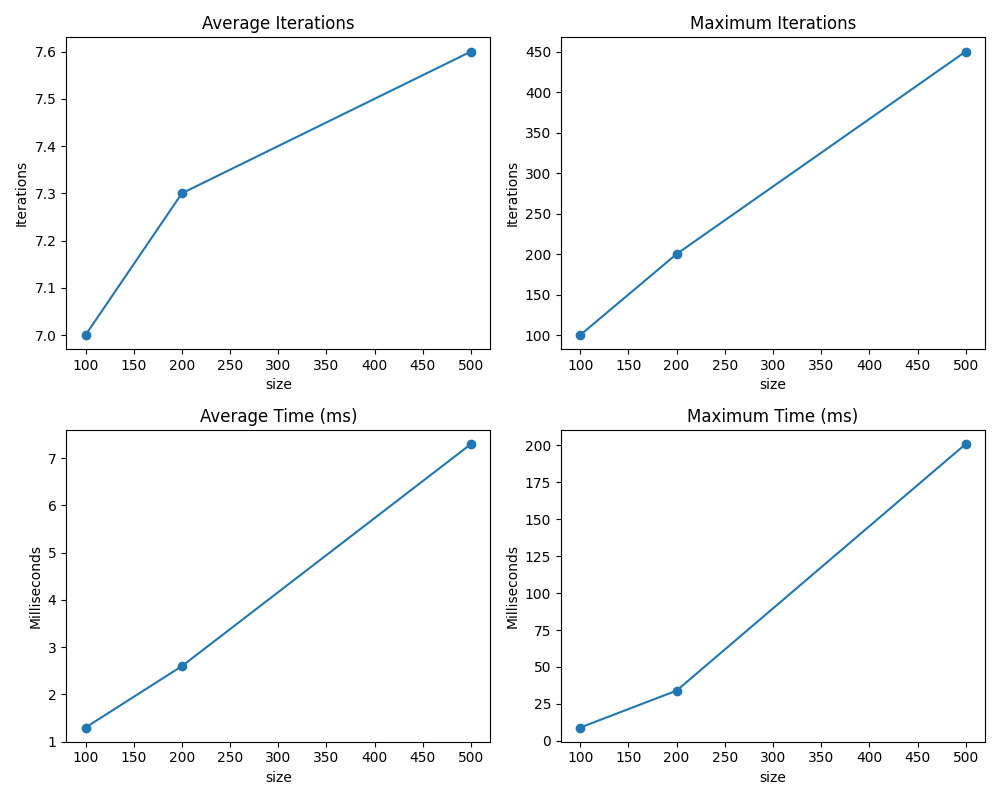
\includegraphics[width=0.8\textwidth]{../common/perf_graphs/e_1.png}
    \caption{Weighted delegation convergence performance with $\epsilon = 1$. Average and maximum iteration counts and convergence times for graph sizes of 100, 200, and 500 voters.}
    \label{fig:e1_perf}
\end{figure}

\subsubsection*{Results ($\epsilon = 0$)}

Under the stricter $\epsilon = 0$ setting (Figure~\ref{fig:e0_perf}), convergence costs increased:
\begin{itemize}
    \item Average iterations were higher, around 21.8 iterations for 500 voters.
    \item Maximum iterations reached the number of voters (500) in worst-case chain graphs.
    \item Average convergence times remained low, scaling linearly with graph size, reaching about 20 milliseconds for 500 voters.
    \item Maximum times reached approximately 225 milliseconds for worst-case chains.
\end{itemize}

\begin{figure}[H]
    \centering
    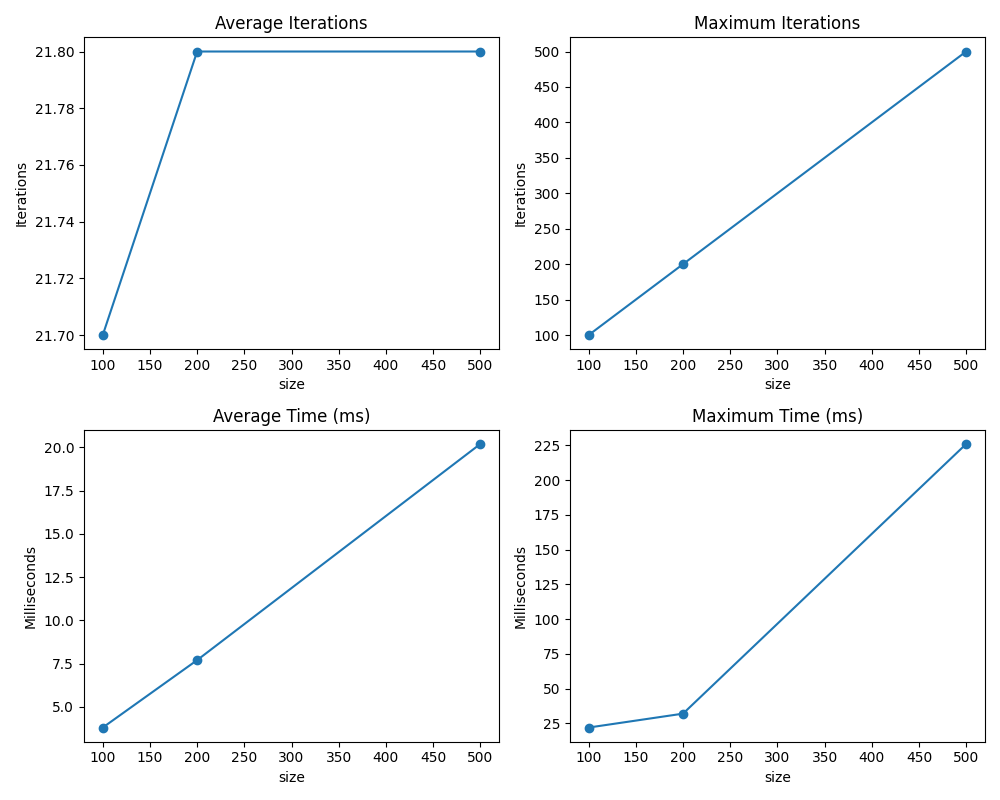
\includegraphics[width=0.8\textwidth]{../common/perf_graphs/e_0.png}
    \caption{Weighted delegation convergence performance with $\epsilon = 0$. Stricter convergence requirements lead to higher iteration counts and slightly increased convergence times.}
    \label{fig:e0_perf}
\end{figure}

\subsubsection*{Discussion}

These results demonstrate that the weighted delegation mechanism scales linearly with the number of voters in typical cases, and remains tractable even in worst-case configurations. Using $\epsilon = 1$ provides a practical trade-off, offering fast convergence without loss of meaningful rating accuracy. Overall, the performance results confirm that the trust matrix model is efficient and suitable for deployment at the intended application scale.

\subsection*{Summary}
Testing confirmed that the delegation features introduced into vodle are resilient, handle both standard and edge cases correctly, and scale efficiently to support realistic deployment sizes. This provides strong evidence for the practical viability of the system in participatory decision-making applications.


\section{Evaluation Against Requirements}

This section evaluates the project against the specific functional and non-functional requirements outlined in Chapter~\ref{ch:project_objectives}. For each project objective, a table summarising whether each requirement was achieved is presented, followed by a detailed discussion providing evidence and references to the implementation. Where necessary, placeholders are included for requirements requiring further confirmation or referencing.

\subsection{Objective 1: Implement a Core Delegation Model}

\begin{table}[H]
\centering
\begin{tabular}{|p{9cm}|c|}
\hline
\textbf{Requirement} & \textbf{Met?} \\ \hline
\textbf{FR1.1:} Users can invite others to act as their delegate & Met \\ \hline
\textbf{FR1.2:} Users can accept delegation requests & Met \\ \hline
\textbf{FR1.3:} Users are prevented from delegating to themselves & Met \\ \hline
\textbf{FR1.4:} Delegation cycles are detected and prevented & Met \\ \hline
\textbf{FR1.5:} Users can view and revoke delegations & Met \\ \hline
\textbf{FR1.6:} Delegations are resolved transitively & Met \\ \hline
\textbf{FR1.7:} Users can override delegated votes & Met \\ \hline
\textbf{NFR1.1:} Delegation data stored as JSON & Met \\ \hline
\textbf{NFR1.2:} Schema changes backward compatible & Met \\ \hline
\textbf{NFR1.3:} Privacy preserved (only final outcomes visible) & Met \\ \hline
\textbf{NFR1.4:} Delegation UI intuitive & Met \\ \hline
\end{tabular}
\caption{Evaluation of Objective 1: Core Delegation Model Requirements}
\label{tab:objective1_requirements}
\end{table}

\subsubsection{Discussion:}

\begin{itemize}
    \item \textbf{FR1.1 and FR1.2:} Achieved through the delegation invitation system, where users generate a secure, unique link to invite another user to act as their delegate (see Section~\ref{subsec:design_core}, Figure~\ref{fig:delegation-flow-accept}). This process includes both sending and accepting a delegation request, ensuring that all delegations are consensual.
    \item \textbf{FR1.3:} This is enforced proactively when accepting a delegation (see Section~\ref{subsec:design_core}).
    \item \textbf{FR1.4:} Cycle prevention is enforced proactively when accepting a delegation (see Section~\ref{subsec:design_core}, Figure~\ref{fig:del-accept-cycle}).
    \item \textbf{FR1.5:} Users can view their current delegation and revoke it by pressing a button (see Figure~\ref{fig:vote_override}).
    \item \textbf{FR1.6:} Delegations resolve transitively, meaning that if A delegates to B and B delegates to C, then A effectively delegates to C unless overridden (Section~\ref{subsec:design_core}).
    \item \textbf{FR1.7:} Toggles are implemented, allowing users to switch between their delegate's and their own vote (see Figure~\ref{fig:vote_override}).
    \item \textbf{NFR1.1 and NFR1.2:} All data is serialised and stored in JSON, example below:
\begin{minted}{typescript}
save_inverse_indirect_map(pid: string, oid: string, val: Map<string, string>) {
const jsonData = JSON.stringify(Array.from(mp.entries(), ([k, v]) => [k, Array.from(v.entries())]));
this._setp_in_polldb(pid, `poll.{pid}.inverse_indirect_map`, jsonData);
}
\end{minted}
    \item \textbf{NFR1.3:} Only the final vote is visible to the delegated voter (see Figure~\ref{fig:vote_override}).
    \item \textbf{NFR1.4:} Only one step is required to initiate (create an invite) or remove (press the revoke button) a delegation.
\end{itemize}

\subsection{Objective 2: Implement Ranked Delegation}

\begin{table}[H]
\centering
\begin{tabular}{|p{9cm}|c|}
\hline
\textbf{Requirement} & \textbf{Met?} \\ \hline
\textbf{FR2.1:} Users can specify up to 3 ranked delegates & Met \\ \hline
\textbf{FR2.2:} Ranked delegation resolution follows MinSum rule & Met \\ \hline
\textbf{FR2.3:} Users can override ranked delegation by direct voting & Met \\ \hline
\textbf{FR2.4:} Users can view, reorder, and revoke ranked delegations & Met \\ \hline
\textbf{NFR2.1:} Data stored as JSON & Met \\ \hline
\textbf{NFR2.2:} UI intuitive & Met \\ \hline
\end{tabular}
\caption{Evaluation of Objective 2: Ranked Delegation Requirements}
\label{tab:objective2_requirements}
\end{table}

\subsubsection{Discussion:}

\begin{itemize}
    \item \textbf{FR2.1:} Users are able to assign up to three delegates in a ranked order when setting up a delegation. Uniqueness is enforced when creating an invite (see Section~\ref{sec:design_ranked_delegation}).
    \item \textbf{FR2.2:} The MinSum rule is used (see Section~\ref{sec:design_ranked_delegation}).
    \item \textbf{FR2.3:} Toggles are implemented, allowing users to switch between their delegate's and their own vote (see Figure~\ref{fig:vote_override}).
    \item \textbf{FR2.4:} Users are provided with a drag-and-drop dialog that allows for reordering and removal of ranked delegates (see Section~\ref{sec:design_ranked_delegation}).
    \item \textbf{NFR2.1:} Has been achieved using the same methods as Objective 1.
    \item \textbf{NFR2.2:} The system automatically selects the most preferred (lowest ranked) available delegate in the invitation dialog, minimising user effort and making the ranked delegation implementation intuitive and easy to understand. (See Section~\ref{sec:design_ranked_delegation}, Figure~\ref{fig:ranked_invite}).
\end{itemize}

\subsection{Objective 3: Implement Weighted Delegation}

\begin{table}[H]
\centering
\begin{tabular}{|p{9cm}|c|}
\hline
\textbf{Requirement} & \textbf{Met?} \\ \hline
\textbf{FR3.1:} Users can delegate to multiple users simultaneously and trust weights sum to no more than 0.99& Met \\ \hline
\textbf{FR3.2 }: Trust matrix model used for final rating calculation & Met \\ \hline
\textbf{NFR3.1:} Weighted delegation calculated client-side & Met \\ \hline
\textbf{NFR3.2:} Data serialised as JSON & Met \\ \hline
\textbf{NFR3.3:} UI provided for adjusting trust weights & Met \\ \hline
\end{tabular}
\caption{Evaluation of Objective 3: Weighted Delegation Requirements}
\label{tab:objective3_requirements}
\end{table}

\subsubsection{Discussion:}

\begin{itemize}
    \item \textbf{FR3.1:} This can be seen in Figure~\ref{fig:weighted_info}.
    \item \textbf{FR3.2:} Invitation dialog was extended to allow users to specify a trust level (from 1 to the amount of trust available to delegate), see Figure~\ref{fig:trust-slider}. The final ratings are calculated using an iterative trust matrix model, ensuring that delegation chains propagate weights correctly while converging rapidly to stable outcomes (Section~\ref{sec:design_per_option_delegation}).
    \item \textbf{NFR3.1:} Weighted delegation is calculated client-side. (See Section~\ref{sec:design_per_option_delegation}.)
    \item \textbf{NFR3.2:} Weighted delegation data is stored using the same method as Objective 1.
    \item \textbf{NFR3.3:} An ``expert mode'' was added for adjusting trust values. (See Figure~\ref{fig:weighted_info}.)

\end{itemize}

\subsection{Objective 4: Implement Per-Option Delegation into Vodle}

\begin{table}[H]
\centering
\begin{tabular}{|p{9cm}|c|}
\hline
\textbf{Requirement} & \textbf{Met?} \\ \hline
\textbf{FR4.1:} Users can assign different delegates per option & Met \\ \hline
\textbf{FR4.2:} Option-specific delegation resolution independent & Met \\ \hline
\textbf{FR4.3:} Users can override delegated votes per option & Met \\ \hline
\textbf{FR4.4:} UI for per-option viewing and revocation & Met \\ \hline
\textbf{NFR4.1:} Data storage remains CouchDB compatible & Met \\ \hline
\textbf{NFR4.2:} UI clearly indicates delegate per option & Met \\ \hline
\end{tabular}
\caption{Evaluation of Objective 4: Per-Option Delegation Requirements}
\label{tab:objective4_requirements}
\end{table}

\subsubsection{Discussion:}

\begin{itemize}
    \item \textbf{FR4.1:} See Figure~\ref{fig:per-option-delegation-sc} and Figure~\ref{fig:per-option-delegation-invite}.
    \item \textbf{FR4.2:} Delegation resolution is performed at the option level (see Section~\ref{sec:design_per_option_delegation}).
    \item \textbf{FR4.3:} This was achieved in a similar manner to Objective 1 (see Figure~\ref{fig:per-option-delegation-sc}).
    \item \textbf{FR4.4:} A detailed information dialog shows active per-option delegations and allows individual revocation, improving transparency and user control (Section~\ref{sec:design_per_option_delegation}).
    \item \textbf{NFR4.1 and NFR4.2:} The user interface clearly indicates option-specific delegations, and data storage follows JSON formatting conventions compatible with CouchDB.
\end{itemize}

\subsection{Extension Objective: Simulate Delegation Mechanisms}

\begin{table}[H]
\centering
\begin{tabular}{|p{9cm}|c|}
\hline
\textbf{Requirement} & \textbf{Met?} \\ \hline
\textbf{FR5.1:} Model individual agents capable of voting, abstaining, or delegating & Not Met \\ \hline
\textbf{FR5.2:} Support multiple delegation mechanisms (standard, ranked, weighted) & Not Met \\ \hline
\textbf{FR5.3:} Allow configuration of simulation parameters (number of agents, etc.) & Not Met \\ \hline
\textbf{FR5.4:} Track and record key metrics (vote concentration, super-voters, etc.) & Not Met \\ \hline
\textbf{FR5.5:} Output simulation results in structured format (CSV/JSON) & Not Met \\ \hline
\textbf{NFR5.1:} Simulation framework must be lightweight and extensible & Not Met \\ \hline
\textbf{NFR5.2:} Use Mesa and Python libraries (NumPy, Pandas, Matplotlib) & Not Met \\ \hline
\textbf{NFR5.3:} Support reproducibility with fixed random seeds & Not Met \\ \hline
\end{tabular}
\caption{Evaluation of Extension Objective: Simulate Delegation Mechanisms Requirements}
\label{tab:objective5_requirements}
\end{table}

\subsubsection{Discussion:}

The extension objective to simulate delegation mechanisms using agent-based modelling was not achieved. As outlined in Chapter~\ref{ch:project_management}, while the frameworks for an agent based simulation was chosen, the implementation was descoped during the development phase due to time constraints.

The complexity and time demands of finalising and refining the core objectives meant that there was insufficient capacity to also build the simulation environment. This prioritisation was necessary to ensure the core deliverables met the required quality standards.

Nonetheless, foundational planning was carried out, and Chapter~\ref{ch:future} outlines how future work could extend the project by implementing a simulation framework based on the Mesa Python library, with a view to exploring delegation dynamics under different mechanisms and network configurations.

Overall, while this extension objective was not realised within the project timeline, it remains a strong candidate for future research and development.


\section{Feedback}
\label{sec:feedback}

\begin{displayquote}
    \textquotedblleft{}
    The added user interface components are well designed and integrate very well with the existing UI and UX.
    
    The implemented back-end logic works seamlessly with the rather complicated existing data management.
    
    One possible issue with the backend logic is that there might occur racing conditions when several delegations are accepted at basically the same time. This should be easily fixable.
    
    All new code is well-structured and follows the style and conventions of the existing code-base.
    
    The different mathematical methods for resolving delegation cycles, especially the weighted one, are well motivated and present a range of good options for users to delegate all or part of their vote to trusted others, without breaching privacy unnecessarily.
    
    Overall, the weighted delegation implementation will likely be rolled out with the next release of the app.
    \textquotedblright{}
    \end{displayquote}
    
\begin{flushright}
\textemdash\ Jobst Heitzig, Main Developer of Vodle and Customer.
\end{flushright}
    

The feedback from Heitzig confirmed that the project successfully achieved its goals. In particular, the new delegation features were assessed as well-engineered and well-integrated into the existing system. Potential race conditions were identified and acknowledged as addressable. Potential strategies for mitigating this issue are discussed further in Section~\ref{ch:future}.

Overall, the feedback indicated that the delegation extension provides a substantial and valuable improvement to the vodle platform.

\subsection{Summary}

The evaluation demonstrates that the delegation features implemented in vodle successfully met the project's functional and non-functional objectives. Testing confirmed correctness and scalability, while feedback from Jobst Heitzig validated both the usability of the user interface and the seamlessness of the backend integration. Although a potential race condition during simultaneous delegation submissions was identified, it was judged to be easily addressable. The extension objective, implementation of agent-based modelling, was not completed due to time constraints but is identified as a priority for future work. Overall, the system achieves its core goals and provides a substantial improvement to vodle's decision-making capabilities.
